\documentclass[14pt, fleqn, a4paper]{extarticle}
\usepackage[T1, T2A]{fontenc}
\usepackage[utf8]{inputenc}
\usepackage[english, russian]{babel}
\usepackage[backend=biber]{biblatex}
\addbibresource{biblio.bib}

\usepackage{style}
\usepackage{geometry}
\usepackage{import}
\usepackage{subfiles}
\usepackage{indentfirst}
\usepackage{tocloft}
\usepackage{xurl}
\usepackage{hyperref}
\usepackage{enumitem}
\usepackage{setspace}
\usepackage{tabularray}
\usepackage{graphicx}
\hypersetup{
    colorlinks,
    citecolor=black,
    filecolor=black,
    linkcolor=black,
    urlcolor=black,
	breaklinks=true
}
\renewcommand{\cftsecleader}{\cftdotfill{\cftdotsep}}

\newcommand{\asection}[2]{
\setcounter{section}{#1}
\addtocounter{section}{-1}
\section{#2}
}

\newcommand{\asubsection}[2]{
	\setcounter{subsection}{#1}
	\addtocounter{subsection}{-1}
	\subsection{#2}
}

\setlength{\parindent}{1cm}

\setlist[description]{style=nextline}

\begin{document}
	\nocite{*}
	\newgeometry{left=3cm, top=1cm, right=1cm, bottom=2cm}
	\begin{titlepage}
		{
			\large
			\fefutitlepage{к проекту}{Программная инженерия}{09.03.03}{Прикладная информатика}{Б9121-09.03.03пикд}{Травка Е.А.}{Блинов Е.Е.}
		}	
	\end{titlepage}
	\tableofcontents
	\clearpage
	\begin{onehalfspace}
		\subfile{parts/annotation.tex}
		\subfile{parts/intro.tex}
		\begin{figure}[H]
			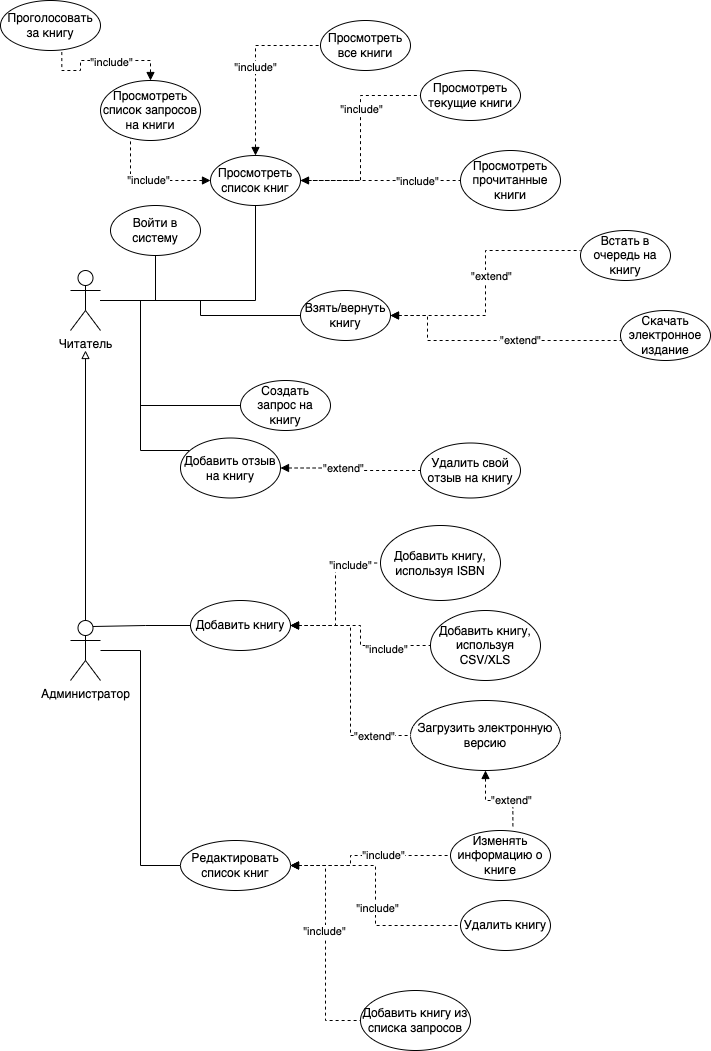
\includegraphics[width=\textwidth]{graphics/usecase-uml.png}	
			\caption{Диаграмма вариантов использования}
			\label{pic:1}
		\end{figure}
		\subfile{parts/functional-needs.tex}
		\subfile{parts/interface-needs.tex}
		\subfile{parts/project.tex}
		\clearpage
		\printbibliography
	\end{onehalfspace}
\end{document}